\section{Segmentation}

Image segmentation is often viewed as the ultimate classification problem, once solved, computer vision is solved. A complete segmentation of an image is a finite set of disjunct regions $R_1, ..., R_n$, such that $I = \bigcup R_i$.


\subsection{Thresholding}

Thresholding is a simple segmentation process, that produces a binary image by labelling each pixel in or out of the region of interest. We do this by comparison of the grey level with a threshold value $T$. Another, better approach can be chromakeying. Hereby we measure the distance from a defined color $g$:

$$I_\alpha = |I - g| > T$$

One limit of thresholding is that it does not consider image context.


\subsection{Segmentation Performance}

If we want to choose the best performing segmentation algorithm or determine a good value for $T$, we need a performance metric. To use automatic analysis, one needs to know the true classification of each test, for this the test images have to be segmented by hand.

One performance metric is the ROC curve. This curve characterizes the error trade-off in binary classification tasks, by plotting the true positive fraction against the false positive fraction. We often choose the operating point on the ROC curve, by assigning cost and values to each outcome:
\begin{itemize}
	\item $V_{\text{TN}}$ - value of true negative
	\item $V_{\text{TP}}$ - value of true positive
	\item $C_{\text{FN}}$ - cost of false negative
	\item $C_{\text{FP}}$ - cost of false positive
\end{itemize}

We then choose the point on the ROC curve with the gradient:
$$\beta = \frac{N}{P} \cdot \frac{V_{\text{TN}} + C_{\text{FP}}}{V_{\text{TP}} + C_{\text{FN}}}$$


\subsection{Pixel Connectivity}

We try to define which pixels are neighbors.

\begin{center}
	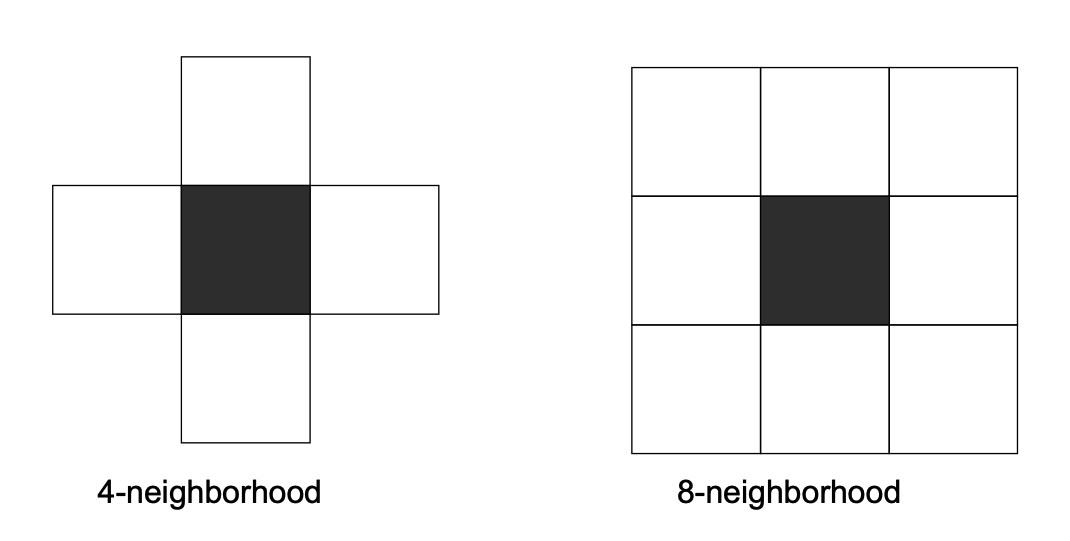
\includegraphics[width=\linewidth]{pixel-neighborhoods.png}
\end{center}

A 4 (or 8) connected path between $p_1, p_n$ is a set of pixels such that every $p_i$ is a 4 (or 8) neighbor of $p_{i+1}$. Now we can defined a region as 4 (or 8) connected if it contains a 4 (or 8) connected path between any two of its pixels.

With this we can introduce \textbf{region growing}. We start from a seed point or region and add neighboring pixels that satisfy the criteria defining a region until we can include no more pixels. There are different approaches to selecting the seed and we could also use multiple seeds. For the inclusion criteria we could choose thresholding or a distribution model.

Another criteria is a snake (active contour). While each point along the contour moves away from the seed, it always has to have some smoothness constraints (minimizing energy function).


\subsection{Distance Measures}

Plain background substraction $I_\alpha = |I - I_{bg}| > T$, where $I_{bg}$ is the background image, we get this by fitting a Gaussian (Mixture) model per pixel. Even better would be:
$$I_\alpha = \sqrt{(I - I_{bg})^\top \Sigma (I - I_{bg})} > T$$

Where $\Sigma$ is the background pixel appearance covariance matrix.


\subsection{Markov Random Fields}

We can add spatial relations with Markov Random Fields (2D Markov Chains).

\begin{center}
	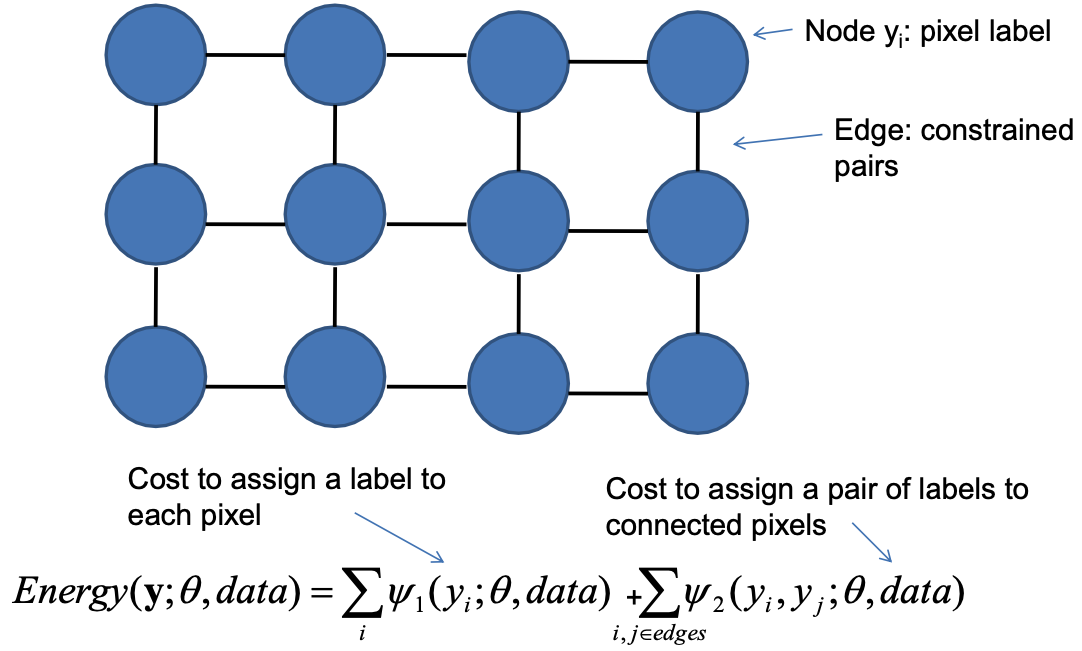
\includegraphics[width=\linewidth]{markov-field.png}
\end{center}

Using a graph cut algorithm we can determine the optimal segementation. We can further optimize this by using iterated graph cut and k-means for learning the colour distribution (GMM) of the image.

\begin{center}
	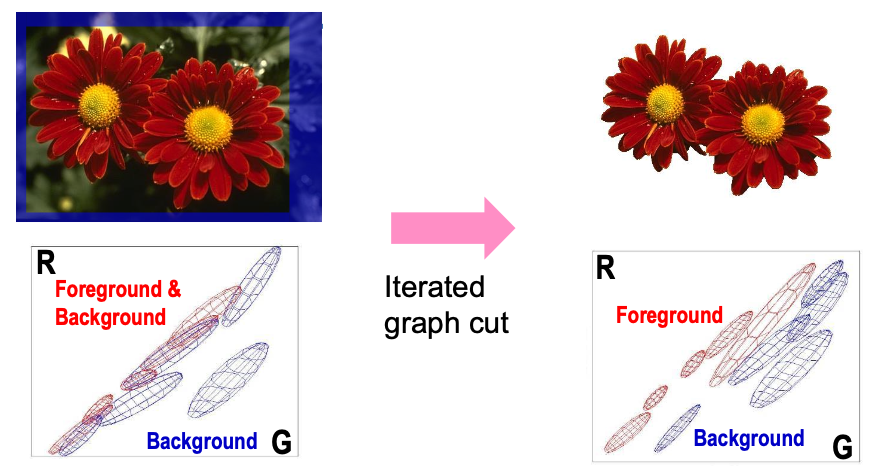
\includegraphics[width=\linewidth]{iterated-graph-cut.png}
\end{center}